% Este archivo es parte de la memoria del proyecto fin de carrera
% de Aarón Bueno Villares. Protegida bajo la licencia GFDL.
%
% Para más información, la licencia completa viene incluida en el
% fichero fdl-1.3.tex
%
% Fuente tomada del PFC 'DSMemorizer' de Diego Barrios Romero, a su vez
% tomada del PFC 'libgann' de Francisco Javier Vázquez Púa, a su vez
% tomada de la plantilla LaTeX para la realización de Proyectos Final
% de Carrera de Pablo Recio Quijano.

% Copyright (C) 2008 Francisco Javier Vázquez Púa
% Copyright (C) 2009 Pablo Recio Quijano
% Copyright (C) 2009 Diego Barrios Romero

% Copyright (C) 2010 Aarón Bueno Villares

\documentclass{article}

\usepackage{./estilos/estiloBase}

\newcommand{\fpt}{\textit{FreePhyloTree }}

\setlength{\parskip}{1em}

\begin{document}

%%%%%%%%%%%%%%%%%%%%%%%%%%%%%%%%%%%%
%%       Preámbulos
%%%%%%%%%%%%%%%%%%%%%%%%%%%%%%%%%%%%
% Este archivo es parte de la memoria del proyecto fin de carrera
% de Aarón Bueno Villares. Protegida bajo la licencia GFDL.
% Para más información, la licencia completa viene incluida en el
% fichero fdl-1.3.tex
%
% Fuente tomada del PFC 'DSMemorizer' de Diego Barrios Romero, a su vez
% tomada del PFC 'libgann' de Francisco Javier Vázquez Púa, a su vez tomada de la plantilla LaTeX para
% la realización de Proyectos Final de Carrera de Pablo Recio Quijano.

% Copyright (C) 2008 Francisco Javier Vázquez Púa
% Copyright (C) 2009 Pablo Recio Quijano
% Copyright (C) 2009 Diego Barrios Romero

% Copyright (C) 2009 Aarón Bueno Villares

\begin{center}

\Large{\textbf{\fpt}} \\
\vspace{.5cm}
\includegraphics[scale=.2]{../../Resources/logo.png}
\vspace{.5cm}

\Large{\textbf{Software de visualización de árboles filogenéticos}} \\

\vspace{1cm}

\huge{\textbf{\underline{Memoria del proyecto}}} \\

\vspace{0.5cm}

\tiny{Aarón Bueno Villares} \\

\vspace{0.5cm}

\end{center}

\tableofcontents

\vspace{12cm}

\begin{center}
\begin{minipage}{15cm}
\rule{15cm}{.3pt}
\\
\tiny{
Este documento ha sido liberado bajo Licencia GFDL 1.3 (GNU Free
Documentation License).\\

Copyright (c) 2010 Aarón Bueno Villares.\\

Permission is granted to copy, distribute and/or modify this document
under the terms of the GNU Free Documentation License, Version 1.3 or
any later version published by the Free Software Foundation; with no
Invariant Sections, no Front-Cover Texts, and no Back-Cover Texts. A
copy of the license is included in the section entitled "GNU Free
Documentation License".
}
\rule{15cm}{.3pt}
\end{minipage}
\end{center}

%\cleardoublepage

%\pagestyle{plain}
%\input{previo}
\cleardoublepage

%\tableofcontents

%%%%%%%%%%%%%%%%%%%%%%%%%%%%%%%%%%%%
%%      Cuerpo
%%%%%%%%%%%%%%%%%%%%%%%%%%%%%%%%%%%%

%\pagestyle{plain}

% Este archivo es parte de la memoria del proyecto fin de carrera
% de Aarón Bueno Villares. Protegida bajo la licencia GFDL.
% Para más información, la licencia completa viene incluida en el
% fichero fdl-1.3.tex

% Copyright (C) 2010 Aarón Bueno Villares

\section{Introducción}
\label{sec:introduccion}

\fpt es \----o pretende ser\---- una herramienta
divulgativa para que estudiantes e interesados en asuntos de biología
evolutiva puedan aprender, la evolución de la vida en la Tierra, tanto
a macroescala como focalizándose en cualquier grupo concreto de organismos
(alguna familia bacteriana, felinos, delfines, hominidos, etcétera).

El proyecto nace en respuesta a varias causas:
\begin{itemize}
\item Ausencia de softwares similares.
\item Deseo de poner en práctica patrones de diseño.
\item Inspiración en el software \textit{gource}.
\item Ganas de aprender a programar bajo librerías 3D.
\item Proyecto de «entrenamiento» para mi posterior proyecto fin de
  carrera, que será un visualizador de algoritmos y modelos de
  computación, en dónde solo trabajaré con primitivas gráficas para
  realizar animaciones, al igual que en \textit{gource} y en
  \textit{FreePhyloTree}.
\end{itemize}

Por todos éstos motivos, decidí inscribirme en el CUSL V, y así tener
un incentivo para poder poner este proyecto en marcha.



\section{Contexto conceptual}
\label{sec:conceptos}

Para comprender bien en qué consiste \fpt para alguien ajeno
a campos como la genética o la evolución biológica, hace falta antes
definir conceptos relacionados y saber exáctamente donde se enmarca el
software. Ésta sección será muy importante ya que es la que describe
la naturaleza del campo en el que está inmerso \fpt lo que nos ayuda a
comprender los problemas y las dificultades \----que se verán en las
próximas secciones\---- contra las que \fpt ha debido, debe y deberá
de enfrentarse para lograr los objetivos marcados.

\subsection{Concepto de evolución}
El concepto de evolución es a veces entendido como una vía de
progreso, desde formas inferiores o peores, a formas superiores o
mejores. En realidad, la \textbf{teoría sintética de la
  evolución}\footnote{También llamado síntesis evolutiva moderna,
  neodarwinismo o sencillamente teoría sintética.} solo se
basa en un \textbf{hecho científico}, a saber, que cualquier par
de organismos tiene un antepasado común. Ésta base tan simple no
permite otorgar ningún tipo de connotaciones de superioridad,
dominancia o dirección a la palabra \textbf{evolución}, que se define,
sencillamente, como sinónimo de \textbf{cambio}.

A grandes rasgos, la evolución funciona de la siguiente forma. Las
características de un individuo \----como la altura, fuerza física o
metabolismo\---- no son más que el reflejo de las
proteinas que existen en tu cuerpo. Como ejemplo, las células de los huesos se
distinguen de las células de la piel, en que las primeras tienen las
proteínas propias de los huesos, y las segundas tienen las proteínas
propias de la piel. Por lo demás, las células serán prácticamente
iguales. ¿Quién tiene la información de qué proteínas debes tener en
tu cuerpo?, pues el ADN, que existe en
cada una de las células de cualquier organismo. El ADN es una cadena larga de
\textbf{bases nitrogenadas}, donde solo ciertas subcadenas son las que
importan: son los llamados genes. Cada gen es un trocito de ADN que
contiene información de una proteina, y estas subcadenas corresponden,
en realidad, una minoría (salvo en bacterias), dado que la mayor parte
del ADN de una célula no sirve para nada\footnote{Ésto no es
  totalmente cierto, pero no entraré en detalles.}. Así, si cambia el ADN,
pueden cambiar tus proteinas, y si ésto ocurre \----es decir, cuando lo
que ha cambiado pertenece a un gen\----, cambian tus
características. Así que la evolución se produce porque el ADN cambia
de generación en generación, por ejemplo, mediante mutaciones (fallo
en la copia de padre a hijo), aunque existen también otros
\textbf{mecanismos de cambio}.

Pero el ADN no cambia completamente, solo cambia una pequeña
parte, y ésta parte no tiene por qué ser la misma, así que los
cambios son muy probables que se hereden a los hijos. Solo hace falta
una cosa: llegar vivo a la edad reproductiva, y además, reproducirse
\----y contra más mejor\----,
y tus nuevas características pueden cambiar la forma en que llegas a
la edad reproductiva y tu tasa de
reproducción. Éste cambio es, \textit{a grosso modo}, selección
natural en el primer caso, y lo segundo es selección sexual. Si tienes éxito
reproductivo, el porcentaje de tu gen, respecto a la población,
crecerá, o disminuirá en caso contrario. Éste porcentaje también puede
cambiar si, en vez de cambiar tus genes, cambia el medioambiente, y lo que
antes era favorable, ahora puede ser perjudicial aunque los genes no
cambien. La selección natural y sexual actuarán de igual aunque los
genes no cambien, pues solo mide como cambia tu éxito
reproductivo. Por eso a éstos mecanismos se les dice que son
mecanismos de \textit{fijación}, ya que la selección
natural\footnote{La selección sexual es, en realidad, un caso
  concreto de selección natural.} acaba por fijar el porcentaje
de ocurrencia de cada gen en la población. Por
supuesto, existen otros mecanismos de fijación además de la selección
natural.

\subsection{Concepto de clasificación}
Antes de que los científicos supieran todo ésto, la visión que se
tenía sobre la biología era muy distinta: los organismos no cambian, y
correspondían a un plan divino, a una «gran cadena del ser» (la
\textit{scala naturae}), en contraposición a la visión evolutiva, que
es un árbol fuertemente ramificado. El hombre estaba en la cima de la
escala biológica, solo por debajo de los ángeles (que ya no pertenece
al mundo biológico), y éste por debajo de Dios. En la base de la
cadena estaban los minerales. Ésta visión estaba tan arraigada que
incluso el concepto de extinción provocaba fuertes conflictos
teológicos.

Debido a que el hombre es la cima de la perfección, el que se parece
más al hombre es más perfecto. Por eso las características de los
individuos eran las que importaban. Especies que se parecen más se
clasificaban juntas. El hombre se clasificaba junto a los monos, los
grandes simios, lemures, colugos (lemures voladores) y
murciélagos, en un órden llamado primates, que significa
primeros\footnote{Los colugos y murciélagos ya no se consideran
  primates.}. Como vemos, la clasificación refleja las ideas de la
época, y antes se clasificaban conforme a las características en
común. Sin embargo, ahora se clasifican conforme a criterios
evolutivos: los que están más emparentados se clasifican juntos.

Las clasificaciones actuales se basan en \textbf{árboles
  filogenéticos}, y aquí ya nos acercamos a lo que \fpt hace. Un árbol
filogenético es un árbol que muestra las relaciones evolutivas entre
un grupo de especies. Cuando un científico quiere establecer saber la
relación evolutiva entre un grupo de especies vivas, hace un estudio
genético y establece sus relaciones, dibujando un árbol filogenético
como el de la siguiente figura, que representa la raíz del árbol
evolutivo de la vida\footnote{Es un árbol desactualizado, la filogenia
  actual de la raíz de la vida ha cambiado drásticamente en los
  últimos años}.

\begin{center}
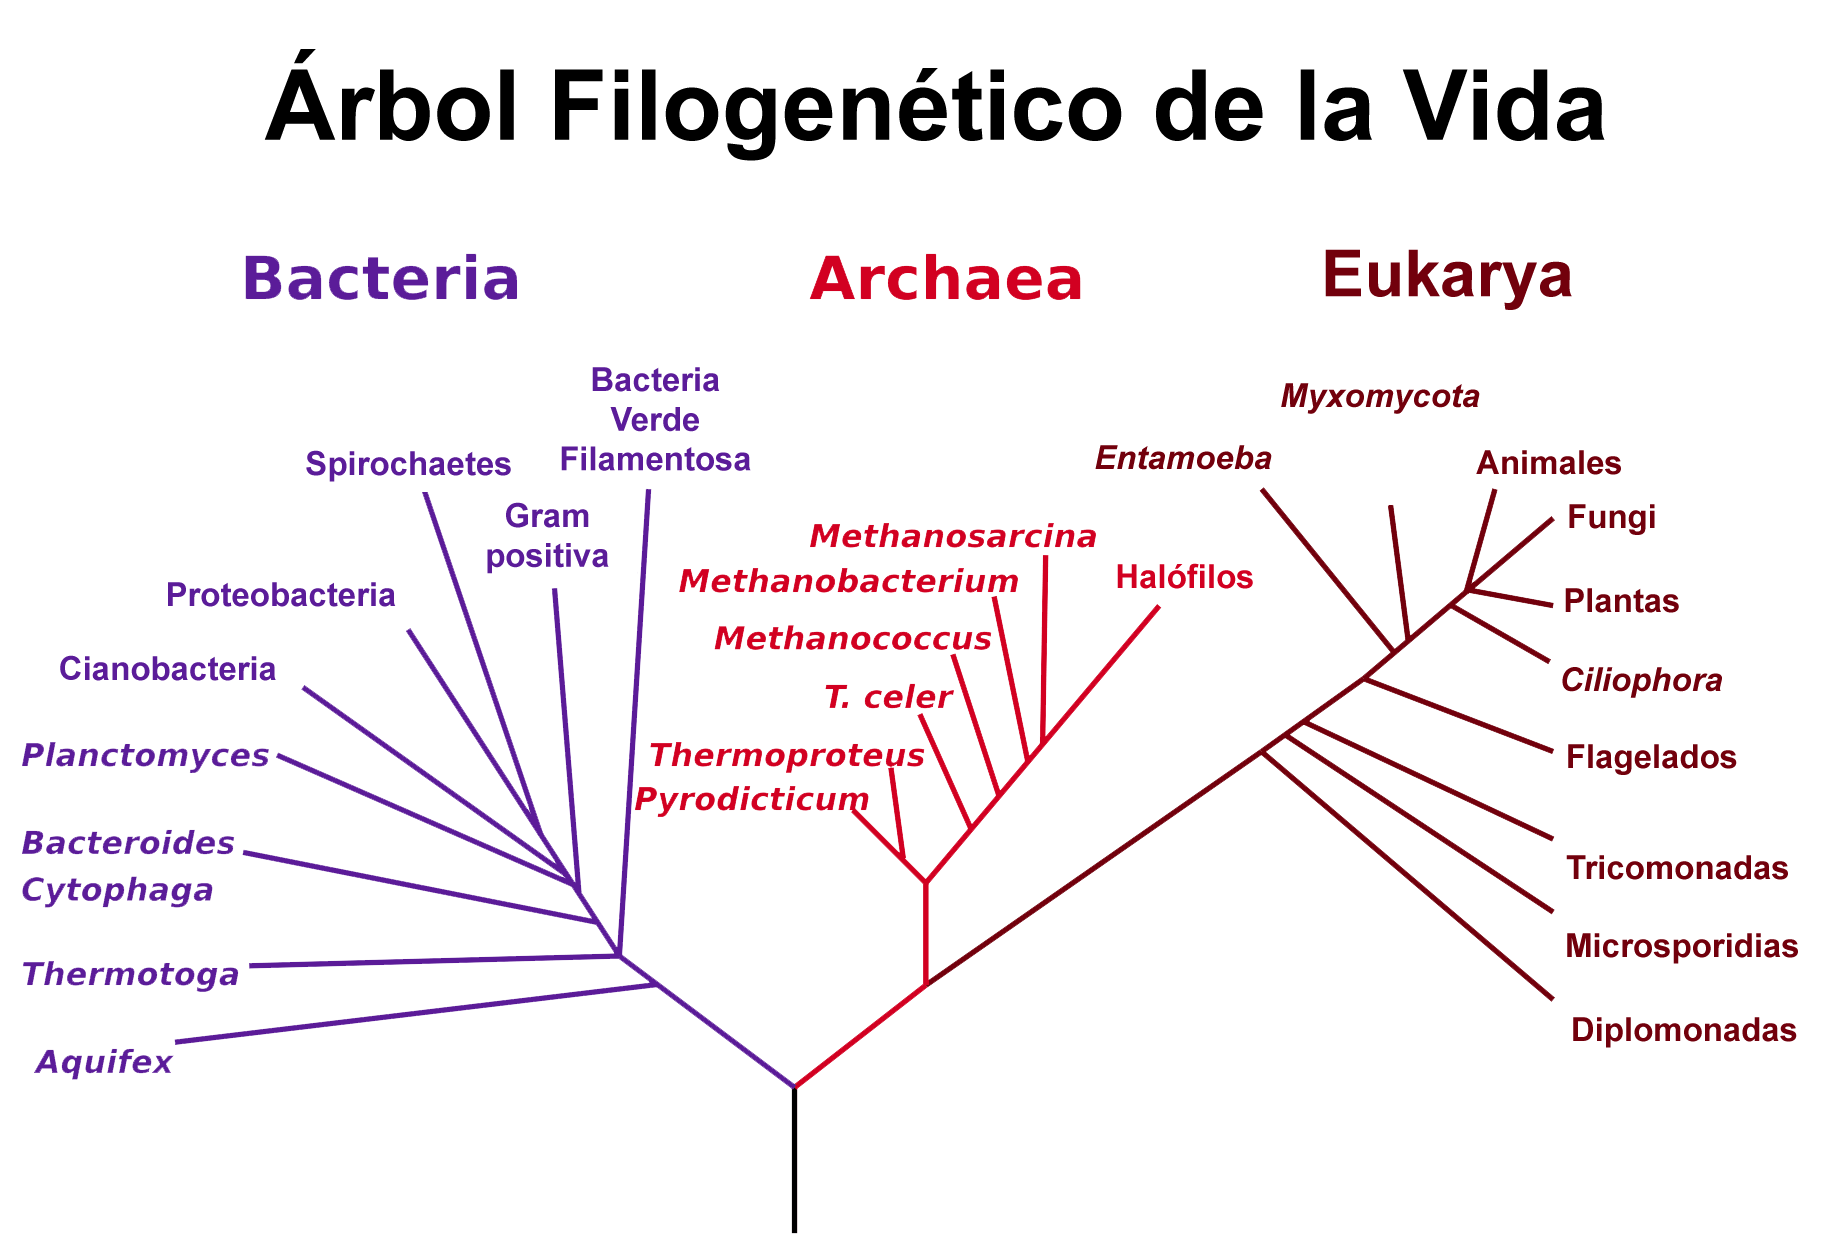
\includegraphics[scale=.2]{images/Phylogenetic_tree-es.png}
\end{center}

En estos árboles, contra más interno sea el nodo, más cercanas son las
especies que agrupa. Por ejemplo, en el árbol anterior se muestra como
los eucariontes (\textit{Eukarya}), son más cercanos a las arqueas
(\textit{Archaea}) que a las bacterias. La clasificación se realiza a
partir de éstos árboles filogenéticos: el árbol filogenético muestra
que especies están más emparentadas, y las especies más emparentadas
se clasifican juntas. Generalmente, la clasificación es una
simplificación de un árbol filogenético, ya que los árboles
filogenéticos son demasiado ramificados como para servir de
clasificación útil y cómoda.

\subsubsection{Taxonomía y sistemática}
En la ciencia de la clasificación hay que distinguir dos subciencias
que hace falta distingüir, por un lado, la \textbf{taxonomía} es la normativa
de clasificación, es decir, las reglas del juego. Ahora, se puede
jugar de muchas formas, es decir, dentro de unas mismas reglas se
puede clasificar a las especies bajo distintos enfoques. Ésto es lo
que se llama \textbf{sistemática}.

Por ejemplo, una regla dada por la taxonomía es: las especies se
clasifican usando dos nombres, el nombre del género, y el nombre de la
especie. Éstos nombres serán en latín, y se escribirán en
cursiva. El nombre del género se escribe comenzando por mayúscula, y
el nombre específico de especie únicamente en minúscula, así, en el
género \textit{homo} existen las especies \textit{Homo sapiens},
\textit{Homo   neanderthalensis}, \textit{Homo ergaster},
etcétera. También existirán, como mínimo, 6 niveles de clasificación:
reino, filo, clase, órden, familia, género y especie. Así, el hombre
pertenece al reino \textit{animalia}, al filo \textit{chordata}, clase
\textit{mammalia}, órden \textit{primates}, familia
\textit{hominidae}, género \textit{homo}, especie \textit{Homo
  sapiens}. También se pueden definir categorías intermedias para
clasificar más cómodamente a grupos muy diversos, como por ejemplo,
subfilo, superórden o infraclase. Cada elemento de la jerarquía de
clasificación se llama \textbf{taxón}. Los reglas para dar nombres a
los taxones se llama \textbf{nomenclatura biológica}.

La sistemática se encarga de definir los criterios bajo los cuales
agrupar y en qué nivel taxonómico incluyo cada grupo. Por ejemplo, las
aves evolucionan a partir de los dinosaurios, por tanto, podrías
incluir a las aves como familia del superórden \textit{dinosauria},
pero también puedes opinar que las aves son un grupo demasiado
diverso y evolucionado como para clasificarse en un nivel tan
específico, y clasificarlas en la clase \textit{aves}. Así, se definen
varias escuelas dentro de la propia sistemática, cada uno con
criterios distintos:

\begin{description}
\item[Fenética:] Clasifica a las especies según la cercanía
  morfológica, tal y como se hacía antigüamente\footnote{Los
    partidarios de la fenética moderna, evidentemente, tienen unos
    criterios totalmente distintos y científicos que los argumentos
    religiosos usados antigüamente.}.
\item[Cladística:] Todo taxón debe incluir a todos sus
  descendendientes, y así, las aves deberían incluirse \textbf{dentro}
  de \textit{dinosauria}. A cada taxón así formado se le llama un \textbf{clado}.
\item[Sistemática evolutiva:] No sólo se usan criterios evolutivos en
  la clasificación, sino también de éxito adaptativo, diversidad,
  etcétera, y así, las aves deberían incluirse en un taxón más alto de
  la jerarquía, y no dentro de \textit{dinosauria} debido a su
  condición de grupo diverso y exitoso por su adaptación a un gran
  número de nichos ecológicos distintos.
\end{description}

Como vemos, la taxonomía y la sistemática son dos ramas relativamente
desacopladas, así, la moderna clasificación basada en criterios
evolutivos se conjuga con las antigüas reglas de clasificación fijista
basada en niveles taxonómicos de filo, órden, etcétera.

Pero como pasa con todo, nada está definido de forma absoluta y sin
estar sustenta a cambios. Las escuelas cladística y la sistemática
evolutiva combaten entre sí buscando el consenso, y hay muchas
alternativas a la clasificación en cada grupo. A su vez, cada rama de
la biología tiene su propio concepto de especie, de subespecie, o
incluso la forma de clasificar; por ejemplo, en botánica, en vez de
usar el nombre de filo, se usa el nivel taxonómico de división como
sustituto. Existe el \textbf{código internacional de nomenclatura
  zoológica}, y también los correspondientes códigos internacionales
de nomenclatura en botánica, de bacterias o el \textbf{comité
  internacional de sistemática de procariotas}. También, en vez de
usar las antigüas reglas de clasificación taxonómica, la web
\textit{PhyloCode} propone una \textbf{nomenclatura filogenética} para
que las clasificaciones sean más cercanas a un árbol filogenético, y
conseguir el objetivo ideal de que cada taxón sea un clado\footnote{Un
  clado es el nombre dado a un \textbf{grupo monofilético} cuando éste
  grupo es un taxón. Un \textbf{grupo parafilético} es aquel que no
  posee a todos los descendientes, como en el caso del taxón
  \textit{dinosauria} cuando no incluye a las aves. Un \textbf{grupo
    polifilético} es aquel que contiene especies de grupos evolutivos
  distintos, como el antigüo grupo de primates, que incluía a los
  murciélagos. Actualmente, los debates se centran en si los taxones
  deberían ser grupos monofiléticos \----cladística\---- o si
  también se permiten grupos parafiléticos \----sistemática
  evolutiva\----. El consenso sí existe en el caso de los grupos
  parafiléticos, que no se permiten.}.

\subsection{Árbol filogenético}
Como hemos dicho antes, elaborar un árbol filogenético comienza
eligiendo las especies a las que se quieren conocer sus relaciones
evolutivas. Mediante estudios genéticos, puede saberse, dado un par de
\textbf{genomas} de dos individuos distintos\footnote{Genoma es el
  conjunto de genes de un individuo} la fecha en la que se produjo la
separación, es decir, la época en la que una población antecesora se
dividió en dos grupos mediante, por ejemplo, \textbf{aislamiento
  reproductivo}, ya que, a partir de ciertas tasas de cambio, el
porcentaje de diferencia representa cantidad de tiempo. A mayor
porcentaje de cambio, más antigüedad del ancestro común a
ambos. También, para estudiar las relaciones de parentesco, se acude
al estudio de las características compartidas o características
exclusivas de cada grupo; éste tipo de estudios se llaman
\textbf{análisis cladístico}.

\begin{center}
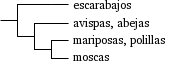
\includegraphics[scale=.7]{images/Cladogram-example1-es.png}
\end{center}

Si son tres especies las que hay que comparar, se compara por parejas
y se crea un árbol con dos escisiones, y así sucesivamente, según el
número de especies. Por eso normalmente los árboles filogenéticos son
dicotómicos, aunque también pueden haber escisiones de más elementos,
como 3 o 4, si no hay mucha diferencia temporal, aunque ésto no suele
ser muy común. A su vez, los árboles filogenéticos pueden tener muchas
apariencias. Los dos árboles filogenéticos adjuntados tienen ya una
apariencia distinta, y la siguiente imágen muestra un árbol
filogenético otra vez completamente distinto.

\begin{center}
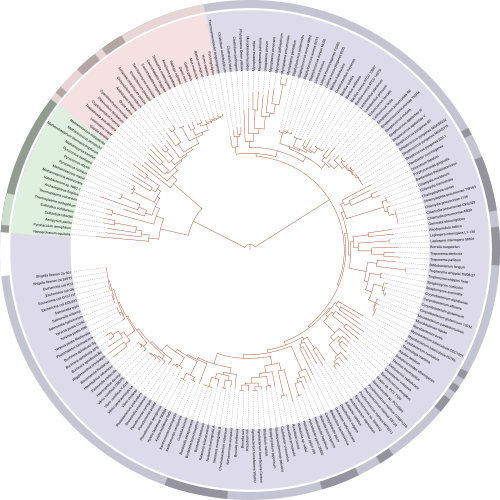
\includegraphics[scale=.7]{images/Tree_of_life.png}
\end{center}

A su vez, los árboles filogenéticos no pueden solamente variar en
forma, sino también en la información que muestra:

\begin{description}
\item[Cladograma:] Un árbol filogenético básico.
\item[Filograma:] Un árbol filogenético donde el tamaño de las aristas
  representa la cantidad de cambio.
\item[Cronograma:] Un árbol filogenético donde el tamaño de las
  aristas representa la cantidad de tiempo evolutivo.
\end{description}

El lector habrá ya advertido la raíz compartida en las palabras
cladística, clado, análisis cladístico y cladograma. El motivo de ésta
sobredominancia del término en tantos lugares distintos tiene un
motivo: el estudio filogenético es la principal vía de clasificación,y
para hacer un estudio filogenético de las especies, el
análisis cladístico es la principal vía de estudio y el resultado es
un cladograma, donde cada subárbol es un clado. Por último, la
cladística transporta éstos cladogramas a la clasificación biológica.
Además, cuando estamos tratando con fósiles y no con especies vivas,
los análisis genéticos no sirven para nada debido a que los fósiles
muy muy rara vez tienen restos de ADN, y si los tienen, éstos son
incompletos, aunque suelen servir. Por todo ésto, la cladística tiene
un papel muy importante en la sistemática biológica, y de ahí la alta
ocurrencia del término en éste documento.

\section{FreePhyloTree y recursos relacionados}
\label{chap:softwares}

\fpt es, actualmente, un visor de la clasificación biológica que, en la
mayoría de los casos, representa un cladograma, aunque no siempre ésto
se cumple, ya que en la clasificación biológica también hay taxones
que son parafiléticos. En un futuro, se espera que la aplicación
visualice árboles filogenéticos, cladogramas, cronogramas y cualquier
tipo de árbol relacionado con la filogenia y la clasificación,
excluyéndo las clasificaciones fenéticas, pues la aplicación siempre
está orientado a estudiar la evolución de las especies\footnote{El
  hecho de incluir en la aplicación información sobre la clasificación
  biológica y no exclusivamente la filogenia, es por un motivo: las
  especies y los grupos evolutivos no se pueden estudiar sino sabes
  como se clasifican, y son dos campos estrechamente unidos,
  \----sobre todo desde que la clasificación se basa en la
  evolución\----}.

\begin{center}
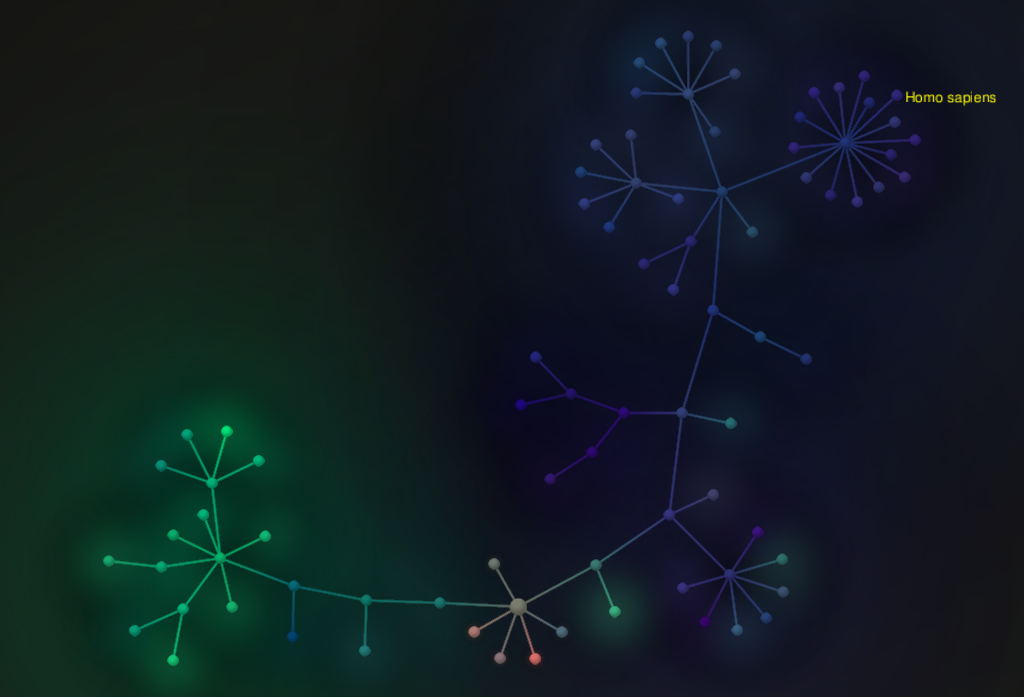
\includegraphics[scale=.5]{../../capture.png}
\end{center}

Ésta es una captura de \fpt. Como vemos, es un árbol que muestra la
clasificación de los primates vista desde el filo
\textit{chordata}, que es la raíz del árbol. La información para
construir el árbol se extrae de \textit{wikispecies}. En la imágen,
\textit{chordata}, se ha expandido dos niveles: se ven sus cuatro
hijos y los hijos de sus hijos. Solo el taxón \textit{vertebrata} se ha
vuelto a expandir. Igualmente, todos los hijos de vertebrata tienen, a
lo sumo, dos niveles de expansión\footnote{El hecho de que sean 2
  niveles es una decisión mía, en compromiso entre la elegancia y
  tiempo de procesamiento, ya que cada expansión requiere una lectura
  al API de \textit{wikispecies}, y a mayor profundidad mayor tiempo
  de lectura, puesto que ésta es recursiva. Con éste equilibrio, el
  usuario nunca tendrá que esperar mucho para que la aplicación
  responda a sus órdenes.}. Nuevamente, el único que hemos vuelto a
expandir ha sido el taxón \textit{tetrapoda}, y así recursivamente
hasta llegar a los primates.

Para terminar de ser una herramienta educativa, hace falta algún
mecanismo de lectura: un texto, documentos o artículos relacionados
con cualquier especie, cualquier concepto o cualquier taxón/clado
presentado, así como mostrar cualquier tipo de información adicional:
como contexto geográfico, climático o temporal. Toda la información
manejada se encapsulará en un wiki, y la aplicación tendrá un
explorador integrado para visualizar los artículos. Sólo con la
lectura puede haber aprendizaje. Para conseguirlo, se ha incrustado un
navegador en la aplicación en la que puede visualizarse el artículo de
\textit{wikipedia} sobre el taxón que deseemos consultar.

Y ésto es todo, lo que por ahora, \fpt hace. Por un lado, puedes
buscar cualquier taxón y ver la clasificación de los subtaxones que
éste contiene, aunque solo en dirección
padre-hijo, pero pronto se podrá explorar la clasificación «hacia
  arriba», es decir, en dirección hijo-padre.

Al lanzar la aplicación, se muestra un menú de ayuda (que puede
ocultarse con F1) con todos los controles existentes, para saber como
expandir o contraer el árbol o como abrir wikipedia.

\subsection{Otros softwares de visualización de taxonomía/filogenia}
Existen otros softwares de visualización de la taxonomía o la
filogenia de las especies, aunque el funcionamiento de éstos softwares
y las bases de datos asociadas participan de todas o algunas de las
siguientes propiedades:

\begin{itemize}
\item El software visualiza árboles filogenéticos a partir de ficheros
  XML. Un fichero XML por árbol filogenético. Éstos ficheros XML
  pueden ser de diversos formatos, y existen estándares \textit{ad
    hoc} sobre el formato de éstos ficheros, que gozan de cierta
  popularidad internacional.
\item Los distintos árboles filogenéticos no se pueden relacionar
  entre sí. Cada fichero es un XML independiente, y no existe ninguna
  base de datos\footnote{Al menos yo no he encontrado ninguna.} que
  contenga una completa clasificación de toda la jerarquía de la
  vida.
\item El software es de corte especializado, y los árboles
  filogenéticos son mostrados o calculados a partir de información
  genética y están diseñadas como herramientas profesionales.
\item Las bases de datos sobre filogenia son sólo de especies vivas,
  ya que para la filogenía de especies fósiles se hace uso exclusivo
  de análisis cladísticos, y éstos análisis no se suman a ninguna base
  de datos global.
\end{itemize}

Existen muchas bases de datos desde distintas universidades u
organismos, pero especializados en ramas concretas o bien necesitan
una licencia para su uso. También existen páginas web, como
\textit{taxonomicon} que almacena información sobre la taxonomía de
muchas especies, mostrando también muchas alternativas según distintos
autores, pero debido a la naturaleza de la página, la información que
allí hay no puede ser usada para montar un software sobre él.

\subsection{Lugares de divulgación relacionados}
\fpt es una herramienta divulgo-educativa, es decir, pretende llegar a
ser una herramienta útil tanto para estudiantes como para
divulgadores. Existen muchos lugares en internet que se dedican a
hacer divulgación científica, desde blogs a wiki, siendo, quizás, la
biología evolutiva la rama más solicitada en divulgación, junto a la
cosmología-astronomía. Como sitios de interés pueden citarse los
siguientes:

\begin{description}
\item[Wikispecies:] Es el wiki usado para construir el árbol de
  \fpt. Ésta página pretende tener actualizada la clasificación más
  moderna y consensuada actualmente, para servir como guía de las
  distintas wikipedias de los distintos idiomas a la hora de crear sus
  correspondientes artículos sobre taxones y/o especies.
\item[Paleofreak:] Blog español sobre paleontología, biología
  evolutiva y temas «afínidos», como el propio autor dice. Es un sitio
  muy visitado y conocido en el mundo de la divulgación científica en
  español, siendo visitado incluso por periodístas, ya que desde ahí
  se hace denuncia de la poca preparación científica de los propios
  periodístas, que suelen publicar noticias llenas de errores
  conceptuales y basadas en prejuicios.
\item[La ciencia y sus demonios:] Otro blog de divulgación donde uno
  de los temas más recurrentes es la biología evolutiva, la
  problemática sobre la religión y la ciencia, etcétera. En algunas
  ocasiones, publican artículos completos dedicados a explicar la
  historia evolutiva de algún grupo biológico en particular.
\item[Palaeos:] Antes sitio web (\textit{palaeos.com}) y ahora wiki
  (\textit{palaeos.org}) basado en la evolución de la vida y de la
  tierra. Sitio web muy interesante con mucha información actualizada
  y excelentes artículos de muchos episodios geológicos y grupos
  biológicos concretos.
\item[Prehistoria universal y vida en la tierra:] Foro en la que se
  abarcan muchos temas, también centrado en biología evolutiva \----aunque
  también hay secciones dedicadas a geología, astronomía,
  etcétera\---- con especial énfasis en la evolución del hombre. Es un
  sitio con poca participación, aunque muchos usuarios y muy
  enriquecido de artículos de muchos temas diversos, del que yo soy
  participante activo y he abierto varios temas, muchos de ellos
  didácticos.
\item[Talkorigins:] Sitio dedicado a discutir sobre el origen
  biológico de las especies o el orígen físico del universo, con un
  carácter ateo-escéptico fuertemente marcado, siendo un lugar también
  muy conocido en el mundo de la divulgación y los debates
  creación-evolución.
\item[Sindioses:] Página de la misma naturaleza que
  \textit{talkorigins} pero en español.
\item[Tree of life web project:] Página web cuyo propósito es mostrar
  la clasificación universal de las especies, y adjuntando artículos
  de cada grupo biológico.
\end{description}

\subsubsection{Propósitos}
Hay muchísimos lugares más, sobre todo blogs, como
\textit{neanderthalensis} o \textit{John Hawks' blog} pero sólo he
resaltado los que considero más importantes y con más repercusión. La
conclusión que hay que sacar es que es un tema con mucho público, hay
muchas personas deseando aprender, y muchas otras deseando enseñar, y
cada página da un enfoque distinto en la medida de sus
posibilidades. \fpt es un intento más de conseguirlo, uniéndo las
ventajas de los softwares y las de la web para suplir las carencias de
uno y otro.

En un futuro, se pretende que la aplicación tenga su propio wiki, con
la información organizada en la forma que \fpt necesita. Es una tarea
titánica hacer de un solo software una herramienta didáctica completa
en éstos campos tan amplios, pero aunando esfuerzos de tanta gente
interesada, y diseñando bien la herramienta de forma que no haya
vacíos que luego los usuarios echen en falta, seguida de publicidad
para que la gente lo conozca, y por último, que guste. La aplicación
se seguirá desarrollando para conseguir todos éstos propósitos y para que
\fpt llege a ser un software de referencia en éstos temas.

También deseo incluir, desde la propia aplicación, un visor gráfico de
toda la información numérica y no exclusivamente textual, como datos
geográficos \----incrustando un mapa y coloreandolo con la
distribución geográfica del grupo en cuestión\----, temporales
\----incrustando una línea temporal y señalando la época en la que
vivió cada grupo\----, la posibilidad de manejar diversas filogenias o
clasificaciones de subárboles, el grado de conversación \----extinto,
en peligro grave de extinción, en peligro leve, etcétera\---- y
cualquier otro tipo de información en forma de datos.

% Este archivo es parte de la memoria del proyecto fin de carrera
% de Aarón Bueno Villares. Protegida bajo la licencia GFDL.
%
% Para más información, la licencia completa viene incluida en el
% fichero fdl-1.3.tex

% Copyright (C) 2010 Aarón Bueno Villares

\section{Historial de desarollo}
\label{sec:desarrollo}

En ésta sección se contarán todas las vivencias acaecidas durante el
desarrollo del proyecto, hasta su estado actual, y un poquito de
cuáles serán los siguientes pasos a dar.

Las versiones publicadas de la aplicación son las versiones desde la
v0.1, v0.2, v0.3, v0.5 y v0.7. A partir de la versión 3, no he tomado
ninguna captura de pantalla, pero puedes ver los videos de cada
versión en youtube, con solo buscar \fpt.

\subsection{En busca de un motor gráfico}
Al comenzar el desarrollo, tuve claro que deseaba hacer algo similar,
en apariencia, a \textit{gource}, pero quizás debido a comentarios
externos, no quise usar openGL pues creía que sería una biblioteca
demasiado difícil de usar. Comencé usando el motor 3D de
\textit{Ogre}, y tras una semana de aprendizaje y agonía, intentando
dibujar primitivas, acabé abandonándo \textit{Ogre} y decidí entrar de
lleno en openGL.

En éste estado, tenía un rudimentario diseño y una simple clase árbol,
que usaba para hacer pruebas. El proyecto, o al menos el día en que
inicialicé el repositorio (creo que inicialicé el repositorio el mismo
día en que comencé a programar) fué el 23 de Octubre del 2010. El 12
de Noviembre ya hice mi primer \textit{commit} en \textit{openGL}. Éste traslado
fue sencillo ya que usé \textit{gource} para aprender a programar en
\textit{openGL}, y éste usaba SDL como gestor de ventanas, librería
que ya conocía. Para imprimir en \textit{gource}, hice uso de
funciones muy básicas para las que no hace falta tener mucha
experiencia, y al día siguiente ya dibujaba un árbol con iluminación
en los nodos, usando los gráficos de gource. La captura que subí al
blog (véase al final) el mismo día fué la siguiente:

\begin{center}
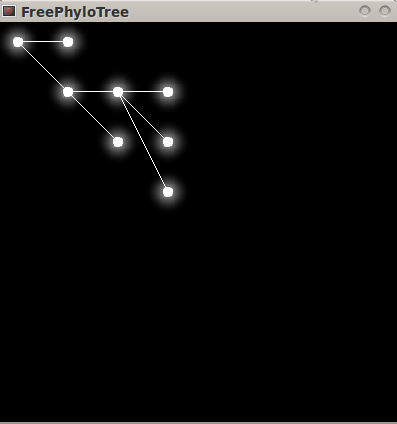
\includegraphics[scale=.65]{images/arbolBlur.png}
\end{center}

\subsection{En busca de un algoritmo de visualización de grafos}
Como vemos en la imágen anterior, los nodos se imprimían con un
primitivo algoritmo de posicionado de nodos. Sencillamente, los hijos
de un nodo se desplazaban a la izquierda unos 50 puntos, y cada
hermano unos 40 puntos en dirección vertical. Los nietos se solapaban
siempre entre sí, y la captura del ejemplo está diseñada para que ésto
no ocurriese.

Estaba claro que me hacía falta un algoritmo de visualización de
grafos, y ésto era una tarea algo más dura. Empecé a documentarme
sobre algoritmos de visualización de árboles, pero ninguna me
convencía, primero, porque no eran algoritmos animables: la posición
de cada nodo se calculaba en un solo paso, y además, los árboles se
imprímian de modo que los hijos se dibujasen, respecto a sus padres,
siguiendo siempre una misma dirección. En la imágen adjuntada arriba, por
ejemplo, los hijos se van imprimiendo en dirección
derecha-izquierda. Yo, repito una vez más, quería visualizar el árbol
tal y como lo hace gource, donde la raíz está en el centro del árbol
con sus hijos a su alrededor, y además, de forma animada.

Lo que hace gource, en realidad, es usar un algoritmo de visualización
general de grafos para visualizar el árbol. Éstos algoritmos siempre
son iterativos, y para conseguir la animación, gource imprime cada uno
de éstos pasos. El algoritmo de visualización que usa gource para
imprimir el árbol es uno basado en quadtrees, y debido a que viendo el
código no comprendía como funcionaba el algoritmo, y buscando en
internet tampoco (además, no sabía que algoritmo concreto usaba
gource), decidí buscar algún documento general sobre visualización de
grafos.

Encontré la tesis doctoral de Andrés Aiello y Rodrigo Ignacio
Silveira, llamado \textbf{Trazado de grafos mediante métodos dirigidos
  por fuerzas: revisión del estado del arte y presentación de
  algoritmos para grafos donde los vértices son regiones
  geográficas}. En ésta tesis doctoral, como dice el título de la
tesis, hay un primer apartado de repaso histórico de los diversos
algoritmos, y el que implementé fué el primer algoritmo que la
historia de la visualización de grafos ha ofrecido: \textit{spring
  embedder}. En el blog (véase al final) hay una entrada completa que
explica en qué consiste dicho algoritmos.

El 27 de Diciembre ya tenía implementado el algoritmo, y sobre el día
30 tenía un algoritmo de coloreado, donde cada nodo se hace cargo de
una región del cubo cromático, y sus hijos van, a su vez,
repartiéndose dicha región, de modo que nodos más cercanos tengan
colores más similares. El 31 de Diciembre fué mi último commit con
SDL, y, en suma, me manejaba con la cámara y podía expandir y contraer
árboles, así como ampliar el radio de destello cuando los nodos se
expande, de forma similar a lo que hace gource. Todas éstas fueron las
características de la versión v0.2.

\subsection{En busca de un explorador integrado}
En la versión v0.2 tenía dos carencias importantes, primero, que
todavía no había explorador integrado y, segundo, que el árbol no se
construía automáticamente, sino que creada los nodos uno a uno desde
el propio código. El siguiente paso era, primero, conseguir el
explorador, para lo que ví la necesidad de usar Qt y desterrar SDL.

Nunca había usado Qt y no sabía como se programaba bajo dicha librería
pero, a decir verdad, la experiencia ha sido muy satisfactoria, puesto
que es muy completo y está muy bien documentado. Tiene un widget
openGL para que allí se renderizen todas las instrucciones openGL, y
también dispone de un widget para mostrar páginas web. Con éste
explorador, en el momento en que el usuario hacia doble click
izquierdo en un nodo, usaba el nombre del taxón para abrir la página
de wikipedia correspondiente, y funcionaba a la perfección sin mucho
esfuerzo. Ésto fué logrado el 14 de Enero del 2011, día en que
publiqué la versión v0.3 de la aplicación, subí un video a youtube y
actualicé el blog.

\subsection{En busca de un nuevo diseño}
\subsubsection{Rama 3D}
En todo éste tiempo, desde que comencé con openGL, he usado varias
fuente para aprender: el libro de openGL, el código de gource y la
inestimable ayuda de Pepe Cullera, al que conocí gracias a una
cuestión sobre el uso de primitivas en Ogre que dejé en el foro
español de Ubuntu, antes de pasarme a openGL. Desde entonces, Pepe me
ha ayudado en muchas ocasiones con openGL.

Tras ver la versión v0.2 del proyecto, le gustó la idea y decidió
desarrollar conmigo. El 15 de Enero se abrió una rama nueva llamada
3ddelopment en la que Pepe Cullera, que domina muy bien openGL,
desarrollara un árbol en 3D, lográndolo en unos 10 días de trabajo.

Debido a que el árbol en 3D, para árboles grandes, no ofrece una
visualización cómoda, y hasta que no se le saque una buena utilidad
(¿quizás para visualizar moléculas orgánicas o genes en un futuro \----muy
lejano por cierto?), no se fusionará con la rama de trabajo
principal.

\subsubsection{Nuevo diseño}
Por mi parte, cambié completamente el diseño de la aplicación,
experimenté con c++0x usando el mecanismo de \textit{variadic
  templates} para manejar una clase vector de un número indeterminado
de dimensiones, así como la directiva \textit{auto} para que el
compilador resuelva por tí el tipo, sin tener que escribirlo
manualmente \----ésto evita tener declaraciones de iteradores
inmensas\----. El mecanismo de plantillas múltiples acabé eliminándolo
debido a que hacía a la ejecución de la aplicación muy lenta. Este
«episodio» de trabajo finaliza el 12 de Marzo.

\begin{center}
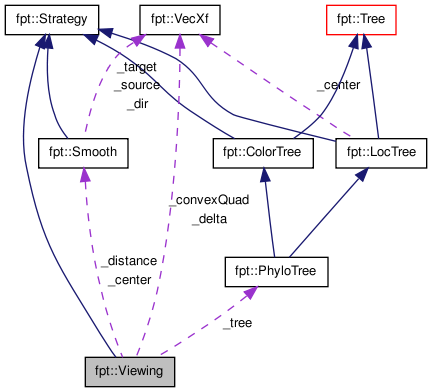
\includegraphics[scale=.65]{images/classDiagram.png}
\end{center}

En el cambio global del diseño, había dos cosas principales que quise
arreglar:
\begin{itemize}
\item La clase árbol tenía demasiada información de diversos aspectos
  que quería desacoplar: información de color, de posición, de ulr's
  de wikipedia, etcétera.
\item Había un comportamiento en común, en muchos puntos del código,
  que quería encapsular: muchos movimientos de la aplicación son
  suavizados, es decir, si un elemento ha de cambiar de posición, no
  cambia de forma brusca, sino suavizada, de modo que el elemento se
  dirige a su nueva posición mediante un parámetro $\delta$ que indica
  el porcentaje de actualización de la posición: un valor $\delta=0.5$
  significa que el elemento, en un solo paso, se mueve la mitad del
  espacio que queda hasta su destino, en su siguiente paso se moverá
  la mitad de lo que quede, y así sucesivamente hasta que esté lo
  suficientemente cerca para finalizar el movimiento. De éste
  comportamiento participan los movimientos de los nodos, sus colores, el
  explorador de wikipedia \----aunque para el explorador ya lo
  quité\----, la cámara, y posteriormente también el buscador que
  añadí y el menú de ayuda.
\end{itemize}

En la imágen adjunta arriba puede verse una parte del esquema del
diseño como ejemplo. La clase \textit{PhyloTree} ahora es la herencia
de un árbol de color y un árbol de posición, que son, a su vez,
árboles. La clase \textit{Viewing}, la responsable de
manejar la cámara, usa la clase \textit{Smooth}, que es la que se
encarga del suavizado de movimientos, ya que la cámara está
suavizada. A su vez, los nodos de color o de posición, que son los que
componen al árbol de color y al árbol de posición también tienen sus
atributos en forma de objetos suavizados.

\subsection{En busca de un cladograma automático}
La segunda gran asignatura pendiente era la construcción automática
del cladograma. Es la recta final de la construcción de la versión
v0.5.

¿Cómo lo conseguí? Pues en un día de intenso trabajo del 14 al 15 de
Marzo. Usé la librería \textit{libcurl}, librería que ya tenía
señalada desde hacía tiempo y ya tenía ciertas nociones de cómo
manejarla, terminé de aprender a usarla, a su vez que aprendía a hacer
consultas al API de MediaWiki. Tuve ciertos problemas con el contexto
de comunicación HTTP desde el software al API, pero con algunos
\textit{googleos} terminé de arreglarlos.

Al principio las consultas se realizaban también contra
\textit{wikipedia} dado que cada artículo tiene una ficha de taxón con
la información de los subclados.

Para hacer éstas consultas, cada taxón tiene en su artículo una
plantilla llamada \textbf{ficha de taxón}. Esta ficha esta siempre
localizada en el mismo lugar del artículo, así que es fácilmente
localizable en el texto. A su vez, los subclados están en un lugar muy
concreto de la ficha del taxón. Lo que no está tan claro es la forma
en que estos subclados son presentados, que varían mucho de taxón a
taxón.

En vista de los problemas que me ocasionaba, decidí construir el árbol
desde wikispecies, porque tengo varias ventajas: el lugar en el que se
encuentran los subclados de un clado dado es igual de claro que en el
caso de wikipedia, y además, la forma en que éstos subclados se
presentan varías mucho menos de taxón a taxón. Además, wikispecies es
más completo y contiene un número muchísimo mayor de taxones, lo que
hace al árbol más completo y al analizador más robusto.

Por último, cabe citar que, a la par que construía el árbol a partir
de wikispecies, también incluí flex como analizador léxico \----antes
buscaba y filtraba el texto a mano. Gracias a flex, ahora el análisis
es mucho más rápido y también es más cómodo extraer los clados. La
versión v0.5 se publicó, como anuncio de todos éstos cambios, el 15 de
Marzo.

\subsection{En busca de una aplicación más completa}
La aplicación tenía ya grandes progresos en funcionalidad, pero había
un campo en el que todavía era un poco pobre, que era la
interactuación con el usuario.

El usuario no sabe qué opciones ofrece el programa cuando lo ejecuta,
ni tampoco tiene opción de explorar directamente un taxón. Cuando se
ejecutaba la aplicación, se cargaba el clado neomura, un clado muy
alto en la jerarquía. Hacían falta más de 15 pasos para llegar al
taxón primates, y el usuario no podía llegar directamente. Ésto era
una carencia importante, y además un problema sabiendo que la fase
final del premio local de Cádiz estaba al caer (martes 22 de
Marzo). Así que añadí un buscador el sábado 20 de Marzo e hice muchos
cambios menores en el código, añadí un documento de README y otro de
INSTALL, actualicé la documentación (sólo las clases) y la página
principal.

Después del concurso, del que salí victorioso, seguí mejorando la
aplicación. Añadí un menú de ayuda donde se ven los controles posibles
de la aplicación, la posibilidad de podar ramas \----quedarte con un
subárbol\----, la posibilidad de fijar nombres de las especies a
voluntad \----antes sólo se visualizaban los nombres cuando ponías el
ratón encima de un nodo\---- y también hice mejoras en cuestión de
eficiencia y cámaras, así como hacer un analizador léxico más robusto,
ya que había taxones que el analizador no reconocía debido a que no
estaban resuelto todos las posibles formas de presentación de los
mismos. Todo ésto me valió una versión v0.7, que cree el 30 de Marzo,
y no publiqué en el blog hasta el día siguiente, día que en que
también hice el último \textit{commit}.

\subsection{En busca de un futuro}
No sé seguro cuál será el siguiente paso a dar, pero en
\textit{wikispecies} hablé de hacer ciertos cambios en la presentación
de los artículos de los taxones para uniformarlos más, y al final la conversación
finalizó por un camino paralelo,
discutiendo sobre algo que no era lo que originalmente proponia y no
ha vuelto a reabrirse, aunque con esa discusión comprendí que sí, que
yo debería tener mi propia wiki.

Luego envíe un correo al blog \textit{la ciencia y sus demonios}
anunciando \fpt, pero no me han contestado todavía. Luego descubrí que
la web \textit{palaeos} había trasladado su página a un wiki, y ese
wiki es lo que más se parece a lo que mi aplicación desea ofrecer, así
que en cuanto tenga tiempo, me pondré en contacto con ellos.


%%%%%%%%%%%%%%%%%%%%%%%%%%%%%%%%%%%%
%%     Desenlace
%%%%%%%%%%%%%%%%%%%%%%%%%%%%%%%%%%%%
%% \backmatter

%% \input{reglamento}
%% \input{manual}

%% %% \nocite{pressman}
%% %% \nocite{laur04}
%% %% \nocite{raym01}
%% %% \nocite{stal04}
%% %% \nocite{mitt04}
%% %% \nocite{sdlweb}
%% %% \nocite{sdlosluca}
%% %% \nocite{cppref}
%% %% \nocite{warh}

%% \clearpage
%% \phantomsection
%% \addcontentsline{toc}{chapter}{Bibliografía y referencias}
%% \bibliographystyle{plain}
%% \bibliography{bibliografia.bib}

%% \input{fdl-1.3}
%% \input{gpl}

\end{document}

%%%%%%%%%%%%%%%%%%%%%%%%%%%%%%%%%%%
%%      Esquema conceptual de la memoria:
%%%%%%%%%%%%%%%%%%%%%%%%%%%%%%%%%%%

%%  Introducción
%%    GoM
%%    Motivación
%%    Sobre este documento
%%  Desarrollo del software
%%    Planificación
%%    Análisis
%%       Especificación de requisitos del sistema
%%              Introducción
%%                        Objetivos
%%                        Alcance
%%                        ¿Qué hace y qué no hace el producto?
%%                        Definiciones
%%              Requisitos generales
%%                        Características del usuario
%%                        Suposiciones y dependencias
%%              Requisitos específicos
%%                        Requisitos de Interfaz de usuario
%%                        Requisitos funcionales
%%                        Requisitos de rendimiento
%%                        Atributos
%%         Modelado de requisitos
%%              Modelo de casos de uso
%%              Modelo conceptual de datos
%%              Modelo de comportamiento del sistema
%%     Diseño
%%       Capa de gestión de datos
%%       Capa de dominio
%%       Capa de presentación
%%     Implementación
%%       Principales problemas de implementación.
%%       Normas de estilo
%%       Documentación
%%     Pruebas
%%     Herramientas utilizadas
%%   Conclusiones
%%     Mejoras futuras
%%              De interfaz
%%              De dominio
%%              De datos
%%     Contacto
%%
%%   Apéndice: Tutorial
%%   Apéndice: Manual de usuario
%%   Apéndice: Reglamento
%%   Apéndice: GFDL
%%
%%   Bibliografía
